\documentclass[lettersize,journal]{IEEEtran}

\usepackage{amsmath,amsfonts}
\usepackage{array}
\usepackage[caption=false,font=normalsize,labelfont=sf,textfont=sf]{subfig}
\usepackage{textcomp}
\usepackage{stfloats}
\usepackage{url}
\usepackage{graphicx}
\usepackage{cite}
\usepackage{xcolor}
\usepackage{balance}
\usepackage{booktabs}
\usepackage{tabularx}
\usepackage{ragged2e}
\usepackage{float}
\usepackage{algorithm}
\usepackage{algpseudocode}



\newcolumntype{Y}{>{\RaggedRight\arraybackslash}X}
\newcolumntype{P}[1]{>{\RaggedRight\arraybackslash}p{#1}}

\newcommand{\status}[1]{\textbf{#1}}

\begin{document}
	\title{Vision-Based Orientation Estimation and Correction for the
	SOFIA Modular Kinetic Surface}
	
	\author{
		Marco Heimdal Castro Magaña, Alejandro Amador Franco, Karen Alejandra Guevara Vasquez, María Alicia Vela Contreras, Juan Pablo Contreras Quiñones,
		Jorge A. Lizarraga, Luis E. González-Jiménez, Luis F. Luque-Vega
		
		\thanks{The authors are with the Department
			of Electronics and Computer Systems,
			ITESO, Tlaquepaque 45604, Jalisco, Mexico.}
	}
	
	
	\markboth{Laboratory for the Development of Technological Solutions}
	{Vision-Based Orientation Estimation and Correction for SOFIA}
	
	\maketitle
	
	
	
\begin{abstract}
    \linelabel{ln:abstract}The SOFIA modular kinetic surface consists of 16 electromechanical modules arranged in a honeycomb configuration, each providing two rotational degrees of freedom through servomotors. 
	Accurate orientation control is essential for coordinated movement, as differences between commanded and actual platform orientations may affect the system's performance. \linelabel{ln:abs-corr}This work presents a vision-based orientation 
	estimation and correction system that uses a neural network to evaluate the physical inclination of the hexagonal platforms. The proposed approach integrates visual perception with the existing embedded control architecture, 
	consisting of an ESP32-C3 microcontroller and PCA9685 PWM drivers. The estimated orientation is compared with the desired reference to determine angular deviations and generate corrective commands for the servomotors. 
	This external feedback mechanism enables the system to adjust platform orientation based on visual measurements rather than relying exclusively on commanded servo positions. The CNN achieved a mean angular estimation error of $0.204^\circ$ and a maximum error of $3.3^\circ$ on the simulated test dataset.
	Additionally, the gesture recognition subsystem was evaluated
	across ten experimental sessions involving two participants
	and 111 recognition attempts. The system achieved an overall
	recognition accuracy of 93.7\%, reaching 100\% under normal
	lighting conditions. Performance decreased under low-light
	conditions, particularly for the ATTACK gesture. Further experimental evaluation is required to quantify residual orientation error and correction performance under physical operating conditions. The study aims to assess the feasibility of visual feedback for improving orientation control in modular kinetic surfaces.
\end{abstract}

	
	\begin{IEEEkeywords}
		\linelabel{ln:keywords}Visual feedback control, orientation estimation, neural networks, computer vision, modular robotics, kinetic surfaces.
	\end{IEEEkeywords}
	
	
	\section{Introduction}
	
	\label{sec:intro}
	
	\IEEEPARstart{S}{OFIA} \linelabel{ln:intro1}is a modular robotic installation composed of 16
	mechatronic units arranged in a two-dimensional honeycomb configuration, with each
	unit providing two rotational degrees of freedom actuated by servomotors. The
	system aims to achieve coordinated control of the multiple actuators while
	enabling interaction through static and dynamic human gestures. For this
	purpose, SOFIA integrates embedded control, inter-module communication, and an
	external computer vision system for gesture recognition.
	
	\linelabel{ln:intro-cap}The SOFIA system requires the
	integration of mechanical actuation, servo control, embedded processing, and
	communication subsystems. \linelabel{ln:intro-32}The complete demonstrator
	requires the coordinated control of 32 actuators through
	multiple PWM signals. The embedded controller must coordinate
	the desired actuator positions, while the communication architecture should
	support the future integration of additional SOFIA modules without
	significantly increasing wiring and control complexity. This work proposes a vision-based approach for angular misalignment diagnosis and closed-loop orientation correction.
	
	\subsection{Problem Statement and Research Question}
	The hexagonal platforms of SOFIA are actuated by low-cost micro-servomotors \cite{sofia_architecture}. Gear backlash, mechanical wear, and accidental manual contact may introduce angular misalignment across the surface, particularly in the absence of external joint feedback. Instrumenting all 16 units with dedicated angle sensors would increase wiring complexity, moving mass, and hardware cost.
	
	\linelabel{ln:rq}To address this limitation, this work investigates the following research question: \textit{Can the two tilt angles of all 16 hexagonal plates be accurately estimated from a single overhead camera to classify each unit without per-module angle sensors?} \linelabel{ln:obj}This encompasses three primary objectives: (1) designing an embedded PCB integrating an ESP32-C3 microcontroller, dual PCA9685 PWM drivers, and RS-485 interfaces to coordinate the 32 actuators; (2) integrating the diagnosis pipeline onto the physical SOFIA module using an overhead camera, four coplanar ArUco markers, and sim-to-real fine-tuning; and (3) integrating state-machine execution with real-time gesture recognition.
	
	\begin{table*}[!t]
		\centering
		\caption{Comparative matrix of related shape-changing interface systems}
		\label{tab:related_work_matrix}
		\scriptsize
		
		\setlength{\tabcolsep}{3pt}
		\renewcommand{\arraystretch}{1.1}
		
		\begin{tabularx}{\textwidth}
			{@{}P{2.2cm} P{3cm} P{3cm} P{4cm} Y@{}}
			
			\toprule
			Reference & Method / technology & Metric / focus & Main result & Gap with respect to SOFIA \\
			\midrule
			
			Relief \cite{leithinger2010relief} &
			Array of 120 motorized pins, scalable low-cost control &
			Actuation density, hardware/software scalability &
			Continuous surface capable of rendering and animating 3D shapes, with per-pin input sensing &
			Translational actuation only (1 DOF per pin); no independent rotation per unit \\
			
			inFORM \cite{follmer2013inform} &
			Pin-based shape display on a pre-existing platform &
			Dynamic physical affordances and constraints, object manipulation &
			Real-time direct-touch interaction and physical rendering of content &
			Same translational limitation as Relief; centralized architecture, not modular per unit \\
			
			TRANSFORM \cite{ishii2015transform} &
			Three large-scale pin displays, kinetic energy as input &
			Aesthetic transformation from static furniture to dynamic system &
			Over one thousand pins coordinated in real-time wave motion &
			Installation-scale system; no per-module orientable control or distributed communication between units \\
			
			PneUI \cite{yao2013pneui} &
			Pneumatically actuated multi-layer soft composite materials &
			Integrated input sensing and shape output in the material itself &
			Four functional applications (phicons, mobile, case, lamp) with controllable shape change &
			Soft/pneumatic actuation, not discrete rotational motion; difficult to scale to precise angular control \\
			
			LineFORM \cite{nakagaki2015lineform} &
			Serial chain of one-DOF servo actuators &
			Line/curve-based interaction affordances &
			Cord, mobile, and body-constraint interfaces through line-shaped actuation &
			Serial (chain) configuration, not a two-dimensional array; 1 DOF per unit, not 2 \\
			
			ChainFORM \cite{nakagaki2016chainform} &
			Identical modules with servo, touch sensing, visual output and embedded processing &
			Hardware modularity and reconfigurability &
			Modular, reconfigurable platform with rich per-module I/O &
			Modularity demonstrated, but still a linear chain, not a 2D array with 2 DOF per node \\
			
			\bottomrule
			
		\end{tabularx}
	\end{table*}
	
	\subsection{Related Shape-Changing Interface Systems}
	\linelabel{ln:rw1}Motorized arrays have been widely explored as a mechanism for generating
	dynamic physical surfaces. Relief introduced an actuated tabletop composed of
	120 individually addressable motorized pins and emphasized a scalable hardware
	and software architecture \cite{leithinger2010relief}. This concept was
	extended through inFORM, where shape actuation was employed to generate dynamic
	physical affordances and constraints and to manipulate physical objects
	\cite{follmer2013inform}. At a larger scale, TRANSFORM explored the
	transformation of static physical structures into dynamic systems driven by
	streams of data and energy \cite{ishii2015transform}. These approaches
	demonstrate the potential of coordinated arrays of actuators, although their
	architectures primarily focus on large pin-based or installation-scale physical
	surfaces.
	
	\linelabel{ln:rw2}Alternative approaches have explored different actuation principles and
	modular configurations. PneUI demonstrated shape-changing interfaces based on
	pneumatically actuated soft composite materials, integrating sensing and active
	shape output within deformable structures \cite{yao2013pneui}. In contrast,
	LineFORM investigated electromechanical shape transformation through serial
	chains of one-degree-of-freedom servo actuators
	\cite{nakagaki2015lineform}. This concept evolved toward greater hardware
	modularity in ChainFORM, where identical modules incorporate motor actuation,
	sensing, visual output, and embedded processing
	\cite{nakagaki2016chainform}. These systems highlight modularity and
	distributed actuation as relevant design characteristics for reconfigurable
	physical interfaces.
	
	\linelabel{ln:rw-tab}The main technological characteristics and differences identified among the
	reviewed shape-changing interfaces are summarized in
	Table~\ref{tab:related_work_matrix}.
	
	\linelabel{ln:gap}In contrast to the reviewed shape-changing interfaces, SOFIA combines a
	two-dimensional honeycomb arrangement with two rotational degrees of freedom
	per unit. Unlike pin-based displays, which predominantly constrain motion to a
	single translational axis, or line-based modular systems organized as serial
	chains, each SOFIA unit can independently modify its orientation while
	remaining part of the same physical surface. This configuration introduces
	design challenges related to coordinated actuation, modularity, scalability,
	control architecture, electrical integration, and communication. Based on the
	reviewed literature, these characteristics were identified as relevant criteria
	for evaluating the technological architecture of the demonstrator.
	Table~\ref{tab:benchmarking} contrasts SOFIA
	with the reviewed solutions using the
	established comparison criteria.
	
	\begin{table}[!t]
		\centering
		\caption{Benchmarking against related shape-changing systems}
		\label{tab:benchmarking}
		\scriptsize
		
		\setlength{\tabcolsep}{2pt}
		\renewcommand{\arraystretch}{1.05}
		
		\begin{tabularx}{\columnwidth}
			{@{}P{1.7cm} P{1.7cm} P{1.5cm} Y@{}}
			
			\toprule
			Solution & Configuration & DOF/ unit & Modularity / scalability\\
			\midrule
			
			inFORM \cite{follmer2013inform} &
			Pin array on fixed platform &
			1 (translational) &
			Low -- centralized control, not designed for modular expansion \\
			
			LineFORM / ChainFORM \cite{nakagaki2015lineform,nakagaki2016chainform} &
			Serial chain of modules &
			1 per module &
			Medium -- modular, but limited to a linear configuration \\
			
			PneUI \cite{yao2013pneui} &
			Pneumatic soft composite material &
			Continuous (non-discrete) &
			Low -- difficult to discretize into individually addressable nodes \\
			
			\textbf{SOFIA (proposed)} &
			2D array, honeycomb modules &
			\textbf{2 (rotational)} &
			\textbf{High -- I2C bus + RS-485 designed for future module expansion} \\
			
			\bottomrule
			
		\end{tabularx}
	\end{table}
	
	\linelabel{ln:opp}From the functional decomposition of the demonstrator and its comparison with
	the literature, several technological opportunities were identified. One is
	the development of a scalable control architecture capable of independently
	coordinating all actuators while reducing the processing load on the main
	controller. Another is the implementation of an inter-module communication
	architecture that allows multiple SOFIA modules to operate as part of a larger
	system. Additional opportunities include the implementation of
	software-defined motion limits and smoothing strategies to prevent abrupt
	servo movements and reduce mechanical stress.
	
	\linelabel{ln:focus}Based on these opportunities, this work focuses on a vision-based misalignment diagnosis methodology for the 16-unit SOFIA array, supported by an embedded electronic and gesture-control architecture. The selected hardware provides the 32-channel PWM generation, wireless telemetry, and differential inter-module communication interfaces required by the demonstrator, while the primary research contribution is the metric overhead rectification and neural-network-based angular estimation evaluated across datasets and prepared for physical module deployment. Automatic Modbus address assignment is outside the experimental scope.
	
	
	\section{Materials and Methods}
	\label{sec:methods}
	
	\linelabel{ln:materials-intro}The SOFIA kinetic surface uses 32 MG90S servomotors for platform actuation \cite{sofia_architecture,mg90s}. Rather than instrumenting individual actuators mechanically, this study evaluates the orientation of all 16 hexagonal platforms simultaneously through an overhead computer vision pipeline.

	\linelabel{ln:hardware-config}The methodology is divided into three main stages: embedded hardware configuration, vision-based rectification with dataset generation in Webots, and comparative evaluation of angular estimation models. The first stage involves the selection and electrical verification of the electronic components required for 32-channel servomotor control and inter-module communication \cite{technical_session}. The second stage establishes an overhead camera calibration procedure using four coplanar ArUco markers to generate metric top-down crops ($1~\text{px} = 1~\text{mm}$) and automates the acquisition of labeled datasets in Webots. The third stage benchmarks a geometric displacement model, a lightweight convolutional neural network (CNN), and a hybrid decision rule to estimate platform tilt angles and classify each unit as \textit{OK} ($<2^\circ$), \textit{REVIEW} ($2^\circ\text{--}5^\circ$), or \textit{MISALIGNED} ($>5^\circ$).
	
	\linelabel{ln:methods-variables}The electronic architecture of the complete SOFIA system includes an ESP32-C3 microcontroller and two PCA9685 PWM drivers, which provide the 32 PWM channels required for actuator control \cite{sofia_architecture,esp32c3,pca9685}.
	
	\linelabel{ln:requirements-intro}The main electrical, communication, and mechanical requirements of the SOFIA demonstrator are summarized in Table~\ref{tab:sofia_requirements}. These requirements are based on the system architecture and the established technical verification criteria \cite{sofia_architecture,technical_session}.
	
	\begin{table}[!t]
		\centering
		\caption{SOFIA Main Requirements}
		\label{tab:sofia_requirements}
		\scriptsize
		
		\setlength{\tabcolsep}{2pt}
		\renewcommand{\arraystretch}{1.05}
		
		\begin{tabularx}{\columnwidth}
			{@{}P{2.1cm} P{2.1cm} Y@{}}
			
			\toprule
			Requirement & Specification & Verification\\
			\midrule
			
			Power &
			5 V servo supply &
			Compatible with MG90S range \\
			
			Logic voltage &
			3.3 V MCU logic &
			Required for ESP32-C3 GPIO \\
			
			Communication &
			WiFi/Bluetooth + I2C &
			Supported by ESP32-C3 \\
			
			PWM control &
			32 servo channels, 50 Hz &
			Two PCA9685 drivers required \\
			
			Mechanical &
			16 modules, 2 DOF each &
			32 servos required \\
			
			\bottomrule
			
		\end{tabularx}
	\end{table}
	
	Figure~\ref{fig:SOFIA_DIAGRAM} \linelabel{ln:sim_architecture} illustrates the system architecture and signal flow of the SOFIA demonstrator. Telemetry and motion commands are communicated wirelessly between a central host PC (connected to a gesture capture camera and an overhead misalignment camera viewing the Master Module framed by four corner ArUco markers) and the Control PCB via Wi-Fi or Bluetooth protocols, while an external 5~V DC power supply feeds the board through a 5~V rail. Onboard processing is handled by an ESP32-C3 microcontroller, which interfaces with two PCA9685 PWM drivers over $\text{I}^2\text{C}$ to control a total of 32 servos. Driver 1 manages channels CH1--CH16 (grey group), while Driver 2 addresses channels CH17--CH32 (blue group, labeled CH1--CH16 on the second module) across the Master Module actuator array. \linelabel{ln:interconn}Interconnectivity between boards is provided through an RS-485 transceiver connected via UART to the ESP32-C3, routing a Modbus bus through JST-PH male and female connectors.
	
	
	\begin{figure}[!t]
		\centering
		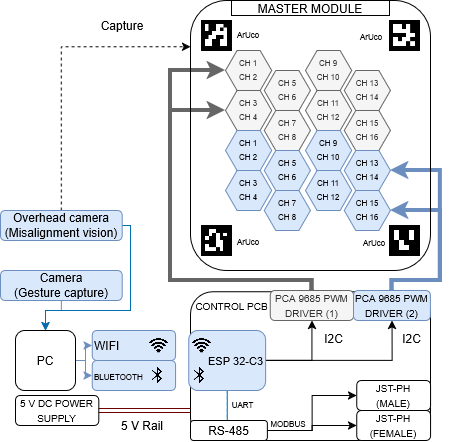
\includegraphics[width=\columnwidth]{figures/SOFIA_DIAGRAM_3}
		\caption{Block diagram describing SOFIA components and connections.}
		\label{fig:SOFIA_DIAGRAM}
	\end{figure}
	
	
	\subsection{Component Specifications and Verification}
	
	The main specifications and design considerations
	for the ESP32-C3, PCA9685, and MG90S are summarized
	in Table~\ref{tab:component_specs}.
	
	\begin{table}[!t]
		\centering
		\caption{Consolidated Component Specifications and
			Design Verification}
		\label{tab:component_specs}
		\scriptsize
		
		\setlength{\tabcolsep}{4pt}
		\renewcommand{\arraystretch}{1.1}
		
		\begin{tabularx}{\columnwidth}{@{}P{2cm} Y Y@{}}
			\toprule
			\textbf{Component} &
			\textbf{Main Specifications} &
			\textbf{Design Considerations / Verification} \\
			\midrule
			
			ESP32-C3
			\cite{esp32c3} &
			Supply: 3.0--3.6 V;
			3.3 V GPIO;
			Wi-Fi 802.11 b/g/n;
			BLE 5;
			strapping pins GPIO2, GPIO8, GPIO9;
			maximum temperature: 105$^\circ$C. &
			Requires regulated 3.3 V supply.
			GPIO inputs must not receive 5 V.
			Boot-pin connections require verification. \\
			
			\midrule
			
			PCA9685
			\cite{pca9685} &
			16 PWM channels;
			12-bit resolution;
			I$^2$C FM+;
			2.3--5.5 V logic supply;
			24--1526 Hz;
			up to 62 addressable devices. &
			Two drivers provide 32 channels.
			Logic supply: 3.3 V;
			PWM frequency: 50 Hz;
			I$^2$C addresses: 0x40 and 0x41. \\
			
			\midrule
			
			MG90S
			\cite{mg90s} &
			Supply: 4.8--6.0 V;
			torque: 1.8--2.2 kgf$\cdot$cm;
			speed: 0.10--0.08 s/60$^\circ$
			at 4.8--6.0 V;
			mass: 13.4 g;
			PWM: 50 Hz. &
			Operates from an external 5 V supply.
			Torque under load requires validation.
			Stall current is not specified
			in the referenced datasheet. \\
			
			\bottomrule
		\end{tabularx}
	\end{table}
	
	
	\subsection{RS-485 Logic-Level Compatibility}\label{sec:rs485_logic}
	
	To enable communication with an additional set of 16 SOFIA
	modules, the proposed architecture incorporates the
	MAX13487E TTL485-V2.0 transceiver module. The MAX13487E
	provides half-duplex RS-485 communication with automatic
	direction control, reducing the need for additional
	transmission-direction control signals \cite{max13487e}.
	
	\linelabel{ln:max5v}According to the manufacturer's datasheet, the MAX13487E
	operates with a nominal 5 V supply, whereas the ESP32-C3
	uses 3.3 V GPIO logic \cite{max13487e,esp32c3}.
	A preliminary electrical test identified a receiver-output
	voltage of approximately 5.00 V at the TXD terminal of
	the TTL485-V2.0 module. This voltage exceeds the
	permitted input range of the ESP32-C3.
	
	\linelabel{ln:rs485-divider}To address this incompatibility, a resistive voltage
	divider was incorporated into the PCB schematic between
	the TTL485-V2.0 TXD output and the ESP32-C3 UART receive
	input. The divider consists of a 10 kOhm series resistor
	and a 20 kOhm resistor connected to ground, producing
	approximately 3.21 V from a nominal 5 V input.
	
	The ESP32-C3 UART transmit output remains directly
	connected to the TTL485-V2.0 RXD input, since the
	MAX13487E specifies a minimum logic-high input voltage
	of 2.0 V \cite{max13487e}.
	
	
	\subsection{Bill of Materials}
	\linelabel{ln:bom-intro}The components required for the SOFIA demonstrator,
	including mechanical parts, actuators, and electronic
	devices, are summarized in Table~\ref{tab:bom}.
	
	
	
	\begin{table}[!t]
		\centering
		\caption{SOFIA Demonstrator Bill of Materials (BOM) Summary}
		\label{tab:bom}
		\tiny
		
		\setlength{\tabcolsep}{1.5pt}
		\renewcommand{\arraystretch}{1.05}
		
		\begin{tabularx}{\columnwidth}{@{}P{0.8cm} P{2.0cm} P{0.5cm} P{0.5cm} P{2.4cm} P{1.1cm} P{0.8cm}@{}}
			
			\toprule
			\textbf{Item} &
			\textbf{Component} &
			\textbf{Qty / Unit} &
			\textbf{Qty / Sys} &
			\textbf{Technical Description} &
			\textbf{Manufacturer} &
			\textbf{Location} \\
			\midrule
			
			1 & Sofia003-P001-03 & 1 & 16 &
			SOFIA module base &
			In-house (LabDST) & ITESO, MX \\
			
			2 & MG90S Servo & 2 & 32 &
			Micro servomotor for module actuation &
			Tower Pro & Hong Kong \\
			
			3 & Sofia003-E002-01 & 1 & 16 &
			Lower joint subassembly &
			In-house (LabDST) & ITESO, MX \\
			
			3.1/4.4 & Pro3 Servo Horn & 2 & 32 &
			Servo output horn for mechanical linkage &
			Tower Pro & Hong Kong \\
			
			3.2 & Sofia003-P004-02 & 1 & 16 &
			Lower joint support, left &
			In-house (LabDST) & ITESO, MX \\
			
			3.3 & Sofia003-P004-03 & 1 & 16 &
			Lower joint support, right &
			In-house (LabDST) & ITESO, MX \\
			
			3.4/3.5/
			4.3/7/8 & M2 Screws & 10 & 160 &
			M2 screws, 10 and 12 mm lengths &
			Walfront & Shenzhen, CN \\
			
			3.6 & Axis 1 & 1 & 16 &
			Joint shaft, 1 mm x 9 mm &
			Mae & Local \\
			
			3.7 & Sofia003-P002-02 & 1 & 16 &
			Lower joint link &
			In-house (LabDST) & ITESO, MX \\
			
			4 & Sofia003-E003-01 & 1 & 16 &
			Upper joint subassembly &
			In-house (LabDST) & ITESO, MX \\
			
			4.1 & Sofia003-P005-01 & 1 & 16 &
			Upper joint support, left &
			In-house (LabDST) & ITESO, MX \\
			
			4.2 & Sofia003-P005-02 & 1 & 16 &
			Upper joint support, right &
			In-house (LabDST) & ITESO, MX \\
			
			5 & Sofia003-P008-01 & 1 & 16 &
			SOFIA top module linkage &
			In-house (LabDST) & ITESO, MX \\
			
			6 & Sofia003-P009-01 & 1 & 16 &
			Top platform support &
			In-house (LabDST) & ITESO, MX \\
			
			9 & M3 Threaded Insert & 1 & 16 &
			M3 threaded insert, 5 mm x 4 mm &
			ZWMSSLL & Shenzhen, CN \\
			
			10 & Sofia003-P000-01 & 1 & 16 &
			SOFIA hexagonal top platform &
			In-house (LabDST) & ITESO, MX \\
			
			\midrule
			
			-- & ESP32-C3 SuperMini & -- & 1 &
			Central microcontroller with Wi-Fi/BLE &
			Espressif (IC) & Shanghai, CN \\
			
			-- & PCA9685 PWM Module & -- & 2 &
			16-channel, 12-bit I2C PWM breakout module &
			Generic (NXP IC) & Unspecified \\
			
			-- & MAX13487E TTL485 & -- & 1 &
			Half-duplex RS-485 transceiver module &
			Generic (ADI IC) & Unspecified \\
			
			-- & RGB LED & -- & 1 &
			RGB status indicator &
			Generic & Local \\
			
			-- & JST-PH Male & -- & 1 &
			2.0 mm-pitch PCB connector for power
			and communication &
			JTAREA & Local \\
			
			-- & JST-PH Female & -- & 1 &
			2.0 mm-pitch mating connector for power
			and communication &
			JTAREA & Local \\
			
			-- & R1--R3 & -- & 3 &
			RGB LED resistors: 330 Ohm &
			Generic & Local \\
			
			-- & R4--R5 & -- & 2 &
			RS-485 voltage divider:
			10 kOhm (R4), 20 kOhm (R5) &
			Generic & Local \\
			
			-- & Regulated DC Power Supply & -- & 1 &
			External regulated 5 V DC supply
			for servomotor power &
			Generic & Local \\
			
			\bottomrule
		\end{tabularx}
	\end{table}
	
	
	\subsection{Justification of Technological Selection}
	
	The selected architecture combines MG90S servomotors,
	two PCA9685 PWM drivers, an ESP32-C3 controller,
	and an RS-485 communication interface. These components
	were chosen to balance actuation requirements,
	PWM channel availability, wireless connectivity,
	and future modular expansion, as summarized
	in Table~\ref{tab:technology_selection}.
	
	\begin{table}[!t]
		\centering
		\caption{Consolidated Technological Selection}
		\label{tab:technology_selection}
		\scriptsize
		
		\setlength{\tabcolsep}{2.5pt}
		\renewcommand{\arraystretch}{1.08}
		
		\begin{tabularx}{\columnwidth}
			{@{}P{1.1cm} P{1.35cm} Y@{}}
			\toprule
			\textbf{Function} &
			\textbf{Selected} &
			\textbf{Alternatives and Rationale} \\
			\midrule
			
			Actuation &
			MG90S &
			Compared with SG90 and MG996R;
			metal gears and favorable
			torque-to-size ratio
			\cite{sg90,mg996r,mg90s}. \\
			
			PWM &
			PCA9685 &
			Compared with software PWM and
			an auxiliary MCU; 16 hardware
			PWM channels over I$^2$C
			\cite{esp32c3,stm32f4,pca9685}. \\
			
			Controller &
			ESP32-C3 &
			Compared with Arduino Nano
			and STM32F4; integrated
			Wi-Fi/BLE and compact design
			\cite{atmega328p,stm32f4,esp32c3}. \\
			
			Comm. &
			RS-485 &
			Compared with direct UART
			and CAN; differential
			multi-drop communication
			\cite{esp32c3,sn65hvd230,max13487e}. \\
			
			\bottomrule
		\end{tabularx}
	\end{table}
	
	
	\subsection{Obtaining Samples for the Vision-Based Misalignment Diagnosis}
	\begin{figure}[!t]
		\centering
		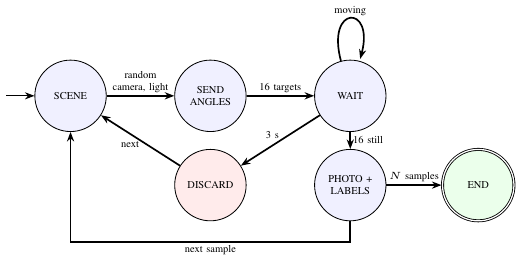
\includegraphics[width=\columnwidth]{figures/Dataset generator}
		\caption{State machine of the dataset generator. A photograph is taken only when the 16 plates report that they reached their target.}
		\label{fig:gen}
	\end{figure}
	\subsubsection{The Photograph}
	
	Four ArUco markers \cite{aruco} are placed around the module at the height of the plates. Using their centers, the photograph is \emph{rectified} to obtain a top-down view with a scale of 1~px per 1~mm. In this view, each plate at its zero-angle position corresponds to a fixed pixel location, allowing a square crop of $128\times128$~px to be extracted around each plate. The 16 crops serve as inputs to the estimation methods.
	
	\vspace{1.5ex}
	\subsubsection{The Generator in Webots}
	
	\linelabel{ln:gen}Taking thousands of real photographs with known angles is not practical, so the images were generated in Webots \cite{webots}, where the angles are known exactly. A supervisor controller and the 16 plate controllers follow the state machine of Fig.~\ref{fig:gen}. For each sample, the supervisor chooses random angles and scene parameters (camera height of 1.30--1.40~m, tilt of up to $\pm4^\circ$, yaw of up to $\pm8^\circ$, lighting, and floor), sends the angles, and waits until all 16 plates report that they are stationary. Only then does it capture the photograph and save the angles \emph{measured} by the joint sensors as labels, rather than the commanded angles. If a plate does not reach its target within 3~s, the sample is discarded. Sample~0, with all plates at their zero-angle positions, serves as the reference.

	\vspace{1.5ex}
	\subsubsection{The First and Second Runs}
	
	Table~\ref{tab:runs} compares the two runs. The second run replaced the simplified plates with the PROTO of the real unit (generated from its CAD model with \texttt{urdf2webots} \cite{urdf2webots}), placed the units as close as possible without collisions, moved the markers closer, used five times as many images, and modified the angular distribution. In the first run, the angles followed a uniform distribution, while the second run represented expected operating conditions, primarily small misalignments with occasional larger deviations caused by manual contact or mechanical obstruction. In both runs, the images were split \emph{by photograph} into training, validation, and test sets, ensuring that all 16 plates from the same photograph were assigned to the same set.

	\begin{table}[!t]
		\centering
		\caption{The Two Runs}
		\label{tab:runs}
		\scriptsize
		\setlength{\tabcolsep}{2pt}
		\renewcommand{\arraystretch}{1.08}
		\begin{tabularx}{\columnwidth}{@{}P{2.0cm} Y Y@{}}
			\toprule
			& First run & Second run\\
			\midrule
			Unit & Simplified plate, 69~mm, arm $L=58$~mm & Real unit (PROTO), 60~mm, arm $L=37$~mm\\
			Markers & 0.76~m square & 0.60~m square\\
			Images (train / val / test) & 2000 (1399 / 300 / 300) & 10\,000 (6999 / 1500 / 1500)\\
			Angles per plate & 5\,\% zero, 50\,\% within $\pm3^\circ$, 45\,\% within $\pm27^\circ$ & 10\,\% zero, 60\,\% up to $5^\circ$, 20\,\% 5--$15^\circ$, 10\,\% $15^\circ$--limit\\
			CNN training & 40 epochs, 84~min & 25 epochs, $\approx$4~h, in parts\\
			\bottomrule
		\end{tabularx}
	\end{table}
	
	\section{Design and Implementation of the Technological Solution}
	\label{sec:design}
	\subsection{Simulation of the 16-Module SOFIA Structure}
	
	Figure~\ref{fig2} \linelabel{ln:sim}shows the simulated response of the SOFIA structure while tracking a moving reference point. The sequence illustrates the reorientation of each module at different instants to maintain alignment with the target.

	\begin{figure}[!t]
		\centering
		\subfloat[Step 1]{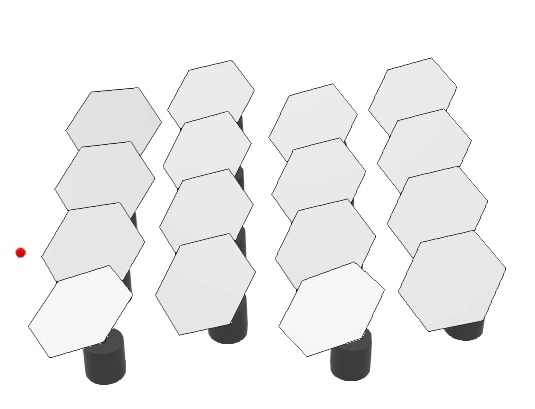
\includegraphics[width=1.1in]{figures/Sim_a}}
		\hfil
		\subfloat[Step 2]{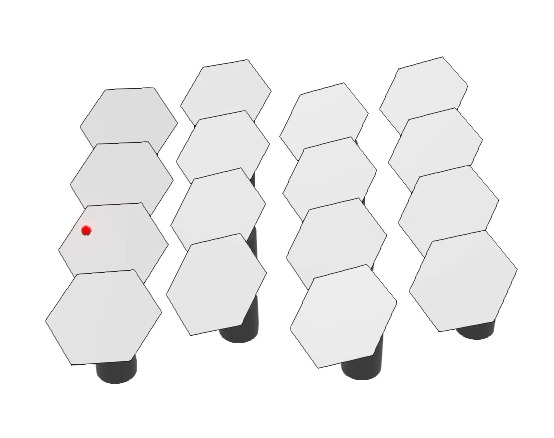
\includegraphics[width=1.1in]{figures/Sim_b}}
		\hfil
		\subfloat[Step 3]{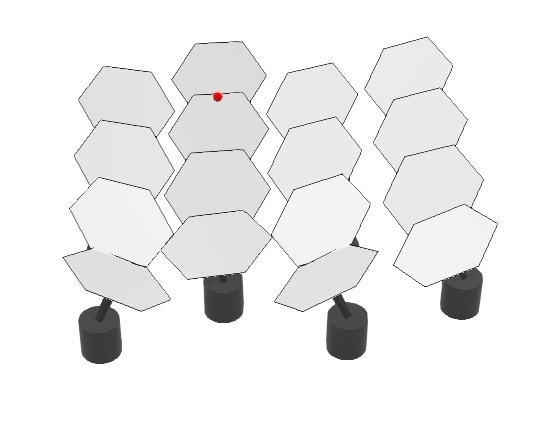
\includegraphics[width=1.1in]{figures/Sim_c}}
		\hfil
		\subfloat[Step 4]{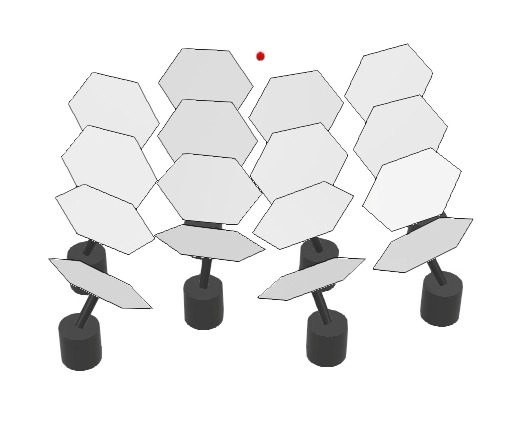
\includegraphics[width=1.1in]{figures/Sim_d}}
		\hfil
		\subfloat[Step 5]{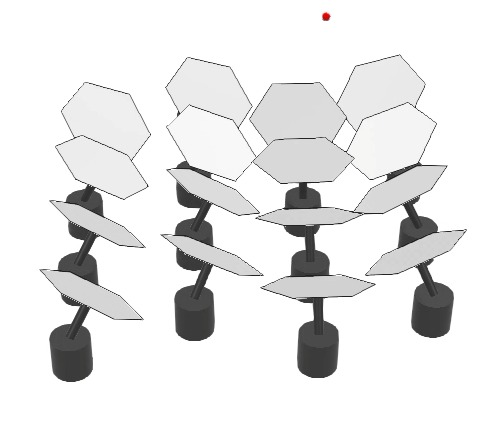
\includegraphics[width=1.1in]{figures/Sim_e}}
		\hfil
		\subfloat[Step 6]{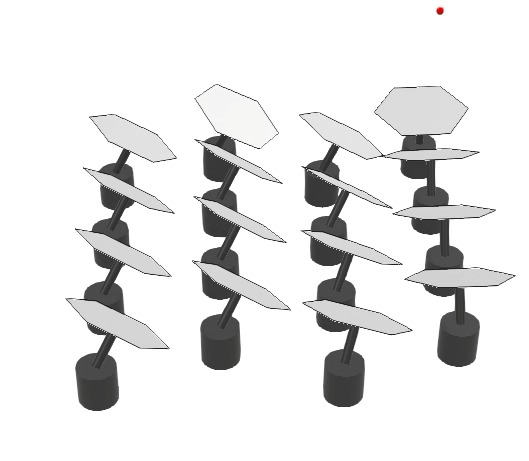
\includegraphics[width=1.1in]{figures/Sim_f}}
		\caption{Simulation of the SOFIA module tracking a moving reference point using inverse kinematics.}
		\label{fig2}
	\end{figure}
	
	Algorithm~\ref{alg:sofia_tracking} \linelabel{ln:alg}summarizes the inverse kinematics and smoothing strategy used by each SOFIA module to orient its platform toward the moving target.
	
	\linelabel{ln:alg1-alpha}In the implemented tracking controller, the EMA smoothing factor in Algorithm~1 was set to $\alpha = 0.25$ at a 50~Hz update rate, attenuating abrupt step changes in target angles.
	
	\begin{algorithm}[!t]
		\caption{SOFIA module target tracking control}
		\label{alg:sofia_tracking}
		
		
		\begin{algorithmic}[1]
			
			\Require Target position $\mathbf{p}$, module base position $\mathbf{r}_{0,2}$, joint limits $[q_{1\min}, q_{1\max}]$ and $[q_{2\min}, q_{2\max}]$, EMA smoothing factor $\alpha \in (0, 1]$
			\Ensure Servo command angles $q_1, q_2$
			
			\State $\mathbf{v} \gets \mathbf{p} - \mathbf{r}_{0,2}$
			\State $\hat{\mathbf{r}}_{2,p} \gets \frac{\mathbf{v}}{\|\mathbf{v}\|} = [u_x, u_y, u_z]^\top$ 
			
			\State $q_1^* \gets \operatorname{atan2}(-u_y, u_z)$
			\State $q_2^* \gets \arcsin(u_x)$ 
			
			\State $q_1^* \gets \Call{ClampAngle}{q_1^*, q_{1\min}, q_{1\max}}$
			\State $q_2^* \gets \Call{ClampAngle}{q_2^*, q_{2\min}, q_{2\max}}$
			
			\State $q_1 \gets q_{1,\text{old}} + \alpha (q_1^* - q_{1,\text{old}})$ \Comment{First-order EMA low-pass filter update}
			\State $q_2 \gets q_{2,\text{old}} + \alpha (q_2^* - q_{2,\text{old}})$
			
			\State Apply $q_1, q_2$ to servo motors
			
			\State \Return $q_1, q_2$
			
		\end{algorithmic}
	\end{algorithm}
	
	\subsection{Mechanical Assembly}
	\linelabel{ln:cad}The mechanical assembly was documented using an exploded
	view generated in SolidWorks, as shown in
	Fig.~\ref{fig:sofia_expl_cad}. The drawing illustrates
	the arrangement of the structural components,
	joint mechanisms, and fastening elements, while the
	accompanying bill of materials identifies their
	part numbers and quantities.
	
	\begin{figure}[!t]
		\centering
		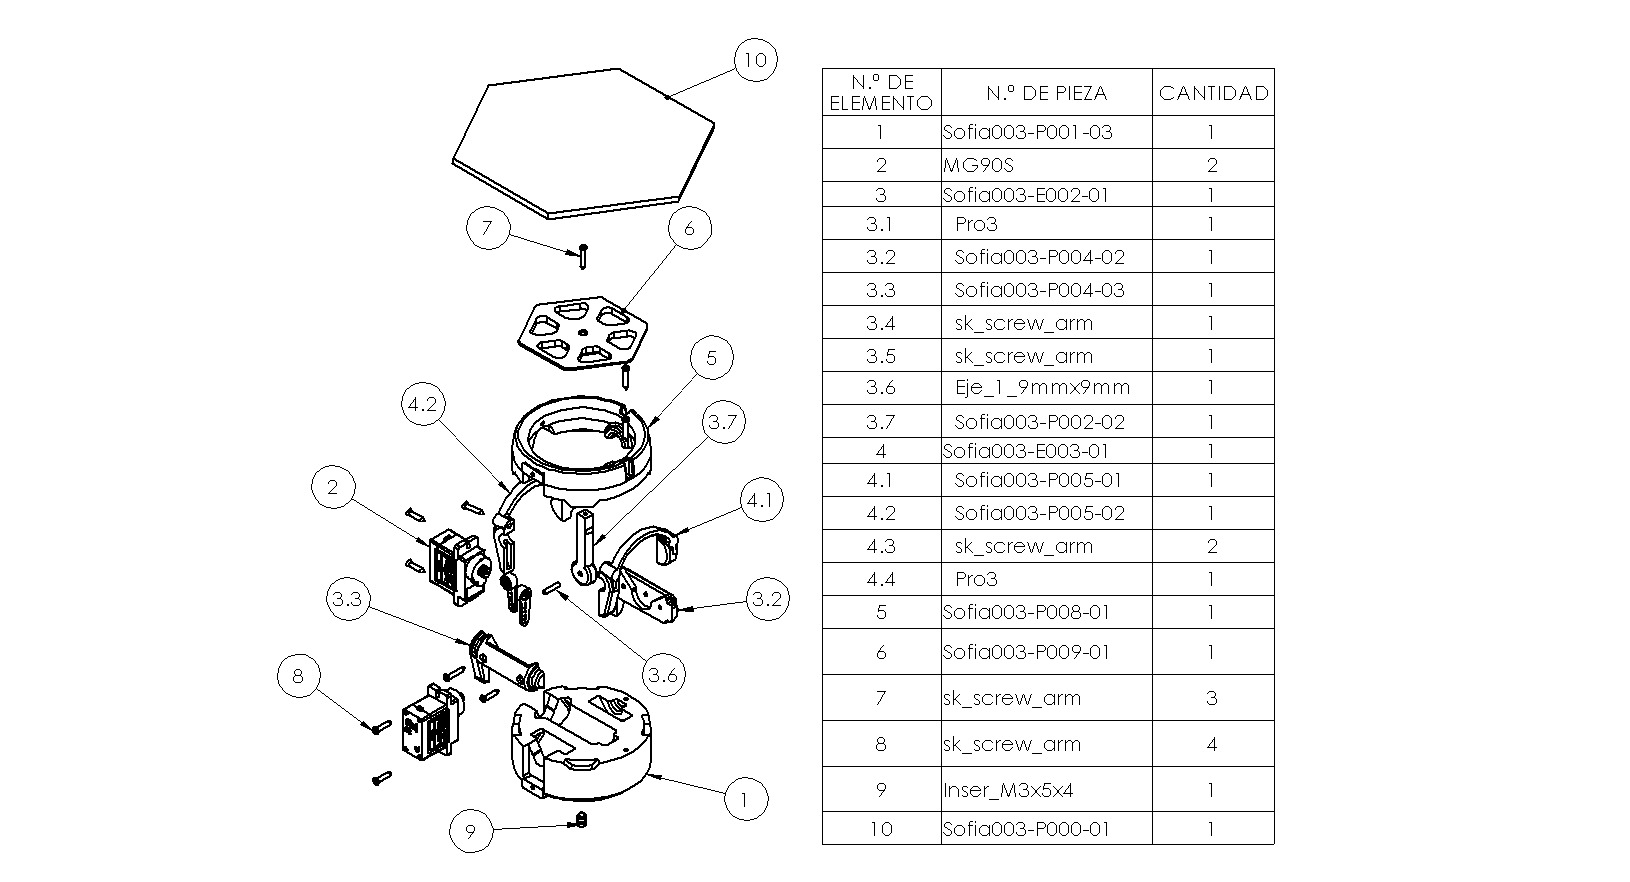
\includegraphics[width=\columnwidth, trim={2cm, 0, 5cm, 0},]{figures/sofia_expl_cad.jpg}
		\caption{Exploded assembly drawing of the SOFIA electromechanical module, including component identification.}
		\label{fig:sofia_expl_cad}
	\end{figure}
	
	\subsection{Methods and Training of the Vision-Based Misalignment Diagnosis}
	
	\subsubsection{Geometric Method}
	
	The geometric method identifies each plate in the top view and measures the displacement of its center relative to the reference position. With the plate at a distance $L$ from the joint axes, the displacement is given by $\Delta v = L\sin\theta_2$ and $\Delta u = L\cos\theta_2\sin\theta_1$, from which both angles are obtained. This method requires no training, but a position error of 1~mm results in an approximate angular error of $1/L$ radians: $1.0^\circ$ with $L=58$~mm and $1.5^\circ$ with $L=37$~mm.

	\vspace{1.5ex}
	\subsubsection{CNN}
	
	A lightweight CNN (five convolutional blocks, 1.28~M parameters) receives one crop and estimates both angles. It was trained in PyTorch \cite{pytorch} using images augmented through mirroring, random lighting variations, and noise to improve generalization. After each epoch, the model is evaluated on the validation images, and only the best-performing model is retained. The test images are used exclusively for the final performance evaluation.

	Since the second run required approximately 4~hours, training was divided into sessions using the state machine shown in Fig.~\ref{fig:train}. The complete training state (weights, optimizer, and learning rate) is saved after each epoch, allowing training to resume from the last saved checkpoint after a time limit or manual interruption.

	\begin{figure}[!t]
		\centering
		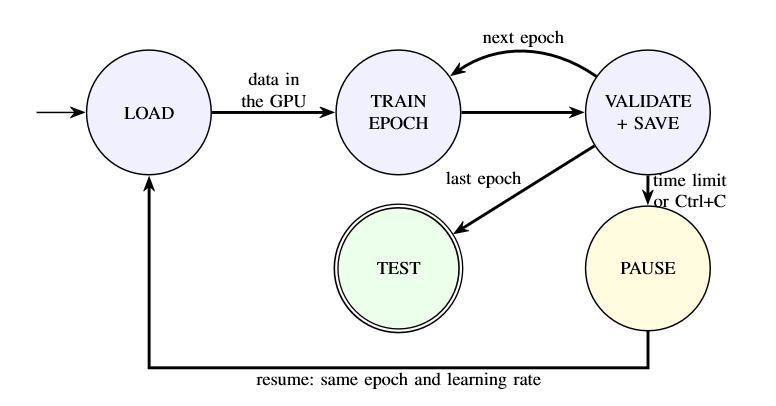
\includegraphics[width=\columnwidth]{figures/State_machine_training}
		\caption{State machine of the training. The state is saved after every epoch, so training can be split into several sessions.}
		\label{fig:train}
	\end{figure}
	
	\vspace{1.5ex}
	\subsubsection{Hybrid Rule}
	
	\linelabel{ln:hybrid}Both methods are evaluated for each plate. If their estimates differ by more than $2^\circ$, the CNN estimate is selected and the plate is marked for inspection. If the estimates agree and the plate is near zero ($\le6^\circ$), the geometric estimate is selected; otherwise, the CNN estimate is used. This rule was developed during the first run, in which the geometric method achieved the highest accuracy near zero.

	\vspace{1.5ex}
	\subsubsection{Exclusion of ResNet18}
	
	\linelabel{ln:resnet}In the first run, a ResNet18 model \cite{resnet} pretrained on ImageNet was also evaluated. Despite having approximately ten times more parameters (13.3~M), it was less accurate than the lightweight CNN (Table~\ref{tab:results_Vision_Train}). This suggests that features learned from ImageNet may offer limited advantages when estimating small pixel displacements. Due to its lower performance and higher computational cost, ResNet18 was excluded from the second run.

	\subsection{Computer Vision Gesture Recognition System Architecture}
	
	\linelabel{ln:intro-vis}The computer vision subsystem of SOFIA recognizes human gestures in real time and translates them into discrete action labels. Using a webcam, the modular Python application captures user movements to enable gesture-based interaction with the robot's control and actuation systems.

	\linelabel{ln:explain-vis}The implementation combines OpenCV for image acquisition and visualization with MediaPipe Tasks for landmark detection. It utilizes two pretrained models—Pose Landmarker (33 body landmarks) and Hand Landmarker (up to two hands with 21 landmarks each)—bypassing custom neural network training by classifying gestures through predefined geometric rules.
	
	\linelabel{ln:model-vis}Organized within the \texttt{Vision/} directory, the modular architecture uses \texttt{main.py} to orchestrate frame capture, model execution, evaluation, and visualization. Landmark detection is handled by \texttt{pose\_detector.py} and \texttt{hand\_detector.py}, while \texttt{gesture\_detector.py} performs classification using \texttt{geometry\_utils.py} for geometric calculations and \texttt{smoothing.py} for temporal stabilization.
	
	\linelabel{ln:model-vis2}Captured BGR frames are converted to RGB for MediaPipe processing. Body landmarks are filtered via an Exponential Moving Average (EMA) to reduce frame-to-frame fluctuations, enabling the system to evaluate normalized distances, joint angles, and relative positions. Hand landmarks are concurrently analyzed to identify specific finger configurations.
	
	\linelabel{ln:model-vis3}The system recognizes five gestures divided into dynamic gestures (START and END, requiring movement sequences over time) and static gestures (RELOAD, SHIELD, and ATTACK, defined by specific body and hand configurations). Once recognized, the interface displays the gesture label, detected landmarks, and a real-time frames-per-second (FPS) indicator.
	
	\linelabel{ln:model-vis4}The perception subsystem is integrated with the ESP32-C3 controller over wireless telemetry, translating recognized gestures into coordinated actuation commands across the 16 physical modules.
	
	\subsection{Geometric Gesture Recognition}
	
	\linelabel{ln:Geo-ges-rec-intro}Gesture classification is based on deterministic rules that use normalized distances, joint angles, relative positions, and movement sequences. This approach keeps the recognition process modular and interpretable.

	\linelabel{ln:Geo-ges-rec2}To reduce the influence of the user's distance from the camera, several geometric measurements are normalized using anatomical references, such as shoulder width and torso height. The normalized distance between two landmarks is calculated as:
	\begin{equation}
		D_{\text{norm}} = \frac{\sqrt{(x_A - x_B)^2 + (y_A - y_B)^2}}{d_{\text{ref}}}
	\end{equation}
	where $A$ and $B$ represent the selected landmarks, and $d_{\text{ref}}$ is the distance between two anatomical reference points.
	
	\linelabel{ln:Geo-ges-rec3}For gestures involving arm positioning, joint angles are calculated using three landmarks. The angle between two vectors, with the elbow as the central point, is defined as:
	\begin{equation}
		\theta = \cos^{-1}\left( \frac{\mathbf{u} \cdot \mathbf{v}}{\|\mathbf{u}\| \|\mathbf{v}\|} \right)
	\end{equation}
	\linelabel{ln:Geo-ges-rec4}These angles are calculated from the two-dimensional projection of the detected landmarks and are used to evaluate arm configurations.
	
	\linelabel{ln:Geo-ges-rec5}The recognition conditions for the five gestures are summarized in Table~\ref{tab:gesture_conditions}.

	\begin{table}[!t]
		\centering
		\caption{Summary of Gesture Recognition Conditions}
		\label{tab:gesture_conditions}
		\vspace{0.5em}
		\begin{tabularx}{\columnwidth}{@{}c l X@{}}
			\toprule
			\textbf{Gesture} & \textbf{Type} & \textbf{Main recognition conditions} \\
			\midrule
			START & Dynamic & Three wrist-to-hip contacts within 3s \\
			END & Dynamic & One raised hand and two horizontal direction changes \\
			RELOAD & Static & Wrists near shoulders, approximately vertical forearms, no two recognized pistol hands \\
			SHIELD & Static & Crossed arms, wrists near opposite shoulders, elbow below shoulders \\
			ATTACK & Static & Elbow angles of 35$^\circ$--125$^\circ$ and two pistol-shaped hands \\
			\bottomrule
		\end{tabularx}
	\end{table}
	
	\linelabel{ln:vision-evaluation}The system evaluates these conditions using the body landmarks estimated by MediaPipe Pose Landmarker and the finger landmarks provided by MediaPipe Hand Landmarker. The resulting geometric conditions are used to determine the recognized gesture, while temporal confirmation mechanisms are applied to improve the stability of static gesture classification.
	
	\subsection{Temporal Filtering and Gesture Validation}
	
	To improve stability, an exponential moving average (EMA) filter is applied to body landmarks using the following equation:
	\begin{equation}
		S_t = \alpha X_t + (1 - \alpha)S_{t-1}
	\end{equation} 
	With $\alpha = 0.3$, the equation becomes:
	\begin{equation}
		S_t = 0.3X_t + 0.7S_{t-1}
	\end{equation} 
	
	\linelabel{ln:five-frame}Additionally, static gestures require confirmation across five consecutive valid frames. During simultaneous activations, the system applies the following priority order: SHIELD, ATTACK, RELOAD, START, and END.

	\subsection{Integration Challenges and Design Refinements}
	
	\linelabel{ln:chal-intro}During development, challenges in landmark stability, gesture overlap, and software integration prompted targeted algorithmic and architectural revisions. To prevent \texttt{AttributeError} crashes when users left the camera frame, missing-landmark validation was added prior to processing. Coordinate fluctuations near recognition thresholds were mitigated by incorporating an EMA filter ($\alpha = 0.3$) alongside a 5-consecutive-frame static confirmation requirement.
	
	\linelabel{ln:chal-reload}RELOAD was converted from a dynamic gesture to a static posture (bent arms, hands near shoulders), refined with constraints on wrist-to-shoulder proximity, vertical bounds, and vertical forearm orientation. 
	To resolve spatial overlap with ATTACK, RELOAD classification is suppressed whenever both hands are detected in a pistol configuration. ATTACK itself was redefined—discarding strict torso proximity, depth restrictions, and an ineffective $90^\circ$–$165^\circ$ elbow range—in favor of a W-shaped posture requiring elbow angles between $35^\circ$ and $125^\circ$, wrists above elbows, and outward hand orientation.
	
	\subsection{PCB Design and Electronic Integration}
	\label{subsec:pcb_design}
	
	\linelabel{ln:pcb}
	A single-layer printed circuit board (PCB)
	was developed as a functional integration
	prototype for the SOFIA modular kinetic
	surface. The board provides the electrical
	interconnections and mounting interfaces
	for an ESP32-C3 SuperMini, two PCA9685
	PWM driver modules, and MAX13487E RS-485
	communication interfaces, as illustrated
	in Fig.~\ref{fig:sofia_schematic}.
	
	The ESP32-C3 communicates with both PCA9685
	modules through the I2C bus, providing
	32 PWM channels for servomotor control.
	The servomotors are powered by an external
	5 V supply, while the RS-485 interfaces
	are intended to support future inter-module
	communication. A resistive voltage divider
	consisting of 10 kOhm and 20 kOhm resistors
	reduces the nominal 5 V receiver output
	of the RS-485 transceiver to approximately
	3.33 V at the microcontroller input.
	
	
	\begin{figure*}[!t]
		\centering
		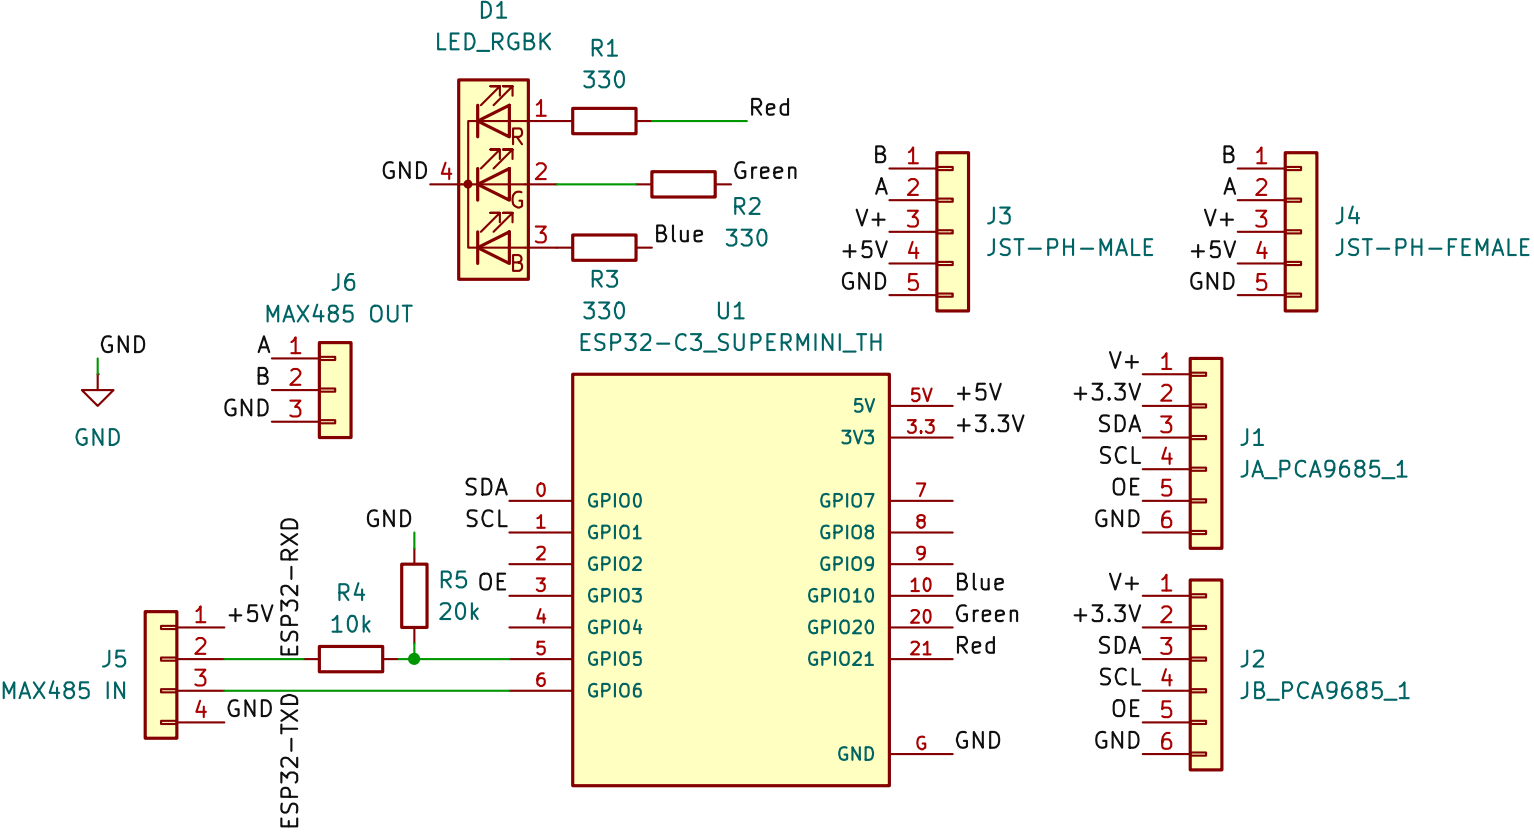
\includegraphics[width=\textwidth]
		{figures/sofia_pcb_schematic.png}
		\caption{Revised electronic schematic of
			the SOFIA control PCB.}
		\label{fig:sofia_schematic}
	\end{figure*}
	
	\linelabel{ln:pcb-traces}
	The PCB layout was developed with 0.7 mm-wide
	traces for power distribution and 0.5 mm-wide
	traces for signal routing. The component
	arrangement, copper routing, and overall
	board dimensions are illustrated in
	Fig.~\ref{fig:sofia_pcb}.
	
	\begin{figure*}[!t]
		\centering
		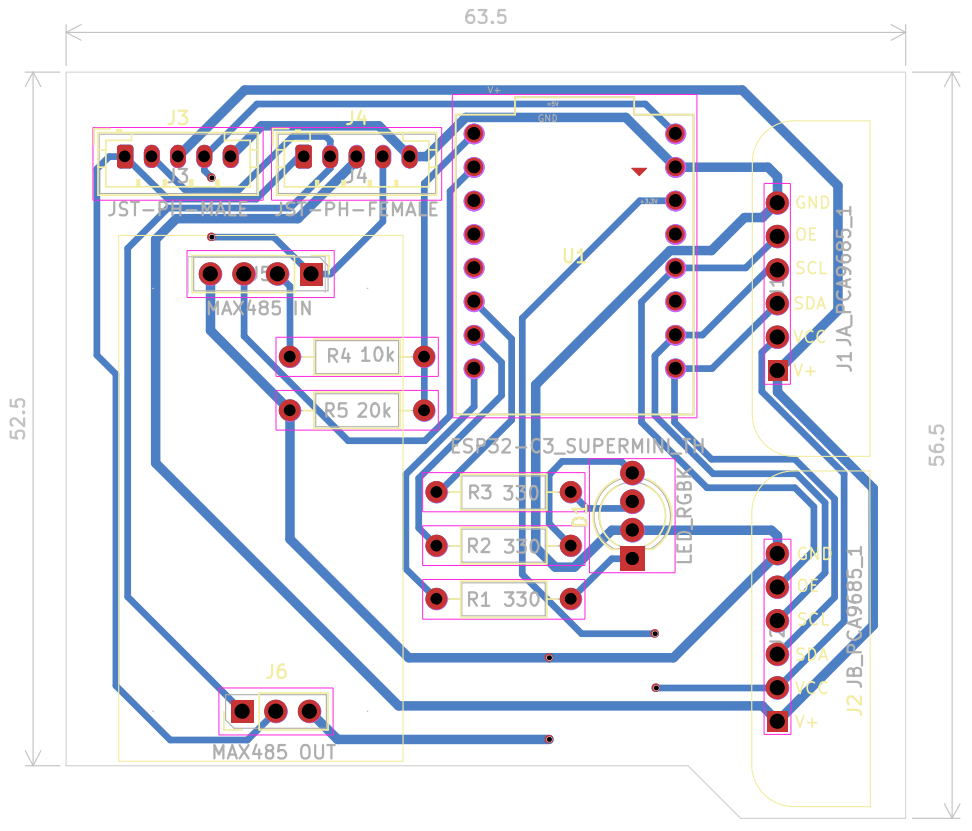
\includegraphics[width=\textwidth]
		{figures/sofia_pcb.png}
		\caption{Single-layer PCB prototype showing
			component placement, copper routing,
			and board dimensions.}
		\label{fig:sofia_pcb}
	\end{figure*}
	
	\subsection{PCB Prototype Limitations}
	\linelabel{ln:pcb-revision}
	The PCB was developed as a functional
	prototype for integrating the SOFIA
	electronic subsystems. However, its
	current-carrying capacity and power
	distribution performance have not yet
	been validated under full system load.
	
	Future work will focus on characterizing
	servomotor current consumption, verifying
	PCB trace and connector ratings, and
	evaluating power distribution and
	decoupling requirements to support
	reliable operation of the complete system.
	
	
	\section{Results}
	\label{sec:results}
	
	\subsection{Preliminary Servomotor Dynamic Response}
	\linelabel{ln:speed}Preliminary speed profiling was conducted on a single module across 12 setpoints ($30^\circ/\text{s}$ to $600^\circ/\text{s}$). The servomotors demonstrated smooth trajectory execution at low-to-medium velocities ($30^\circ/\text{s}$--$350^\circ/\text{s}$). Beyond $500^\circ/\text{s}$, mechanical chatter and motion desynchronization were observed. Based on these preliminary tests, $350^\circ/\text{s}$ was selected as the operating limit for smooth servomotor actuation.

	\subsection{Results for the Training Methods of Vision-Based Misalignment Diagnosis}
	
	\linelabel{ln:res-cnn}Table~\ref{tab:results_Vision_Train} shows the error on the test images of each run (300 and 1500 photographs). The two test sets are not the same, since the unit and the distribution of angles changed, so the comparison is between the two complete setups.
	
	\begin{table}[!t]
		\centering
		\caption{Test Error ($^\circ$) and State Accuracy}
		\label{tab:results_Vision_Train}
		\scriptsize
		\setlength{\tabcolsep}{2.5pt}
		\renewcommand{\arraystretch}{1.08}
		\begin{tabularx}{\columnwidth}{@{}Y c c c c c@{}}
			\toprule
			Method & Mean & Max & $0$--$5^\circ$ & $>15^\circ$ & States\\
			\midrule
			\multicolumn{6}{@{}l}{\textit{First run (simplified plates, 2000 images)}}\\
			Geometric & 0.539 & 74.0 & \textbf{0.13} & 1.30 & 97.2\,\%\\
			CNN & 0.248 & 4.4 & 0.18 & \textbf{0.36} & 96.3\,\%\\
			ResNet18 & 0.293 & 4.1 & 0.21 & 0.43 & 95.9\,\%\\
			Hybrid & \textbf{0.223} & 4.4 & \textbf{0.13} & \textbf{0.36} & \textbf{97.2\,\%}\\
			\midrule
			\multicolumn{6}{@{}l}{\textit{Second run (real unit, 10\,000 images)}}\\
			Geometric & 0.521 & 5.9 & 0.33 & 1.60 & 94.1\,\%\\
			CNN & \textbf{0.204} & \textbf{3.3} & \textbf{0.17} & \textbf{0.41} & \textbf{96.8\,\%}\\
			Hybrid & 0.329 & \textbf{3.3} & 0.33 & \textbf{0.41} & 94.1\,\%\\
			\bottomrule
		\end{tabularx}
	\end{table}
	
	\textbf{First run.} Each method exhibited different strengths. The geometric method was the most accurate near zero ($0.13^\circ$), but occasionally produced large estimation errors (up to $74^\circ$) when a highly tilted plate was confused with an adjacent one. The CNN maintained a lower maximum error ($4.4^\circ$). The hybrid rule combined the advantages of both methods and achieved the lowest mean error ($0.223^\circ$).

	\textbf{Second run.} The CNN achieved a mean error of $0.204^\circ$ and a maximum error of $3.3^\circ$ across 24\,000 plate samples, outperforming the other methods in overall mean error. The geometric method became less accurate near zero ($0.13^\circ \rightarrow 0.33^\circ$) because the shorter arm of the real unit reduces displacement per degree, increasing the impact of pixel-level errors. However, its maximum error decreased to $5.9^\circ$. Consequently, the hybrid rule ranked second in overall mean error ($0.329^\circ$), as it relies on the geometric estimate near zero. Its inspection flags also showed limited reliability: 873 of the 901 flags corresponded to errors of the geometric method rather than the CNN. The CNN was therefore selected as the default method, while the geometric method remains an alternative when a GPU is unavailable.

	\linelabel{ln:findings}Two main findings were identified. First, increasing the number and realism of training images improved CNN performance despite the more challenging geometry. Second, changes in the module geometry may require model retraining, as the CNN from the first run achieved an error of $1.6^\circ$ when evaluated on the second unit configuration.

	\subsection{Functional Validation of the Vision Gesture Recognition Subsystem}
	
	\linelabel{ln:res-func-intro}The computer vision subsystem was tested through real-time webcam experiments to verify its ability to recognize the five predefined gestures. The tests focused on body and hand landmark detection, geometric gesture classification, and temporal validation.
	
	\linelabel{ln:vision-vis}The system successfully captured and processed video frames using OpenCV and MediaPipe, displaying the detected landmarks, recognized gesture labels, and approximate FPS in real time.
	
	\linelabel{ln:vision-func-tests}Functional tests confirmed the recognition of START through three consecutive hand-to-thigh movements and END through two horizontal direction changes of a raised hand. For static gestures, SHIELD was recognized through crossed-arm positioning, RELOAD through the defined arm configuration near shoulder height, and ATTACK through the combination of W-shaped arms and two pistol-shaped hands.
	
	\linelabel{ln:vision-func-ema}The implementation of EMA filtering and five-frame temporal confirmation maintained the functionality of the recognition system while providing mechanisms to reduce unstable detections. Additionally, the final adjustments to RELOAD and ATTACK were verified, confirming that the updated gesture definitions could be recognized during functional testing.
	
	\linelabel{ln:vision-func-summary}These functional tests
	confirmed the operation of the five-gesture recognition
	subsystem. A subsequent quantitative evaluation was
	conducted across ten experimental sessions, including
	111 recognition attempts with two participants under
	different lighting conditions, camera distances, and
	multi-person scenarios. The corresponding recognition
	performance and limitations are presented in the
	following subsection.

	\subsection{Gesture Recognition Performance Evaluation}
	
	\linelabel{ln:res-vision-intro}A new experimental evaluation
	of the gesture recognition subsystem was conducted on
	November 18, 2026, using two participants across ten
	sessions and 111 recognition attempts. The experiments
	evaluated five predefined gestures under different
	camera distances, lighting conditions, and the presence
	of additional people. Each trial started with a visual
	signal, after which the participant performed the
	requested gesture. Recognition was confirmed after five
	consecutive valid frames. The tests were performed on
	Linux using Python 3.14.8, OpenCV 5.0.0, and MediaPipe
	Pose Landmarker and Hand Landmarker.

	
	\linelabel{ln:vision-performance}As shown in
	Table~\ref{tab:gesture_benchmark}, the system correctly
	recognized 104 out of 111 attempts, achieving an overall
	recognition accuracy of 93.7\%. Five of the ten sessions
	achieved 100\% accuracy. START and END reached 100\%
	recall, while RELOAD and SHIELD achieved 95.5\% and
	95.7\%, respectively. ATTACK showed the lowest
	performance, with 77.3\% recall. Overall, six gestures
	were not detected and one was incorrectly classified.

	\begin{table}[!t]
		\centering
		\caption{Final Gesture Recognition Performance}
		\label{tab:gesture_benchmark}
		\footnotesize
		\setlength{\tabcolsep}{5pt}
		\renewcommand{\arraystretch}{1.1}
		\begin{tabular}{@{}l c c c c@{}}
			\toprule
			\textbf{Gesture} &
			\textbf{Trials} &
			\textbf{Hits} &
			\textbf{Recall (\%)} &
			\textbf{Processing (s)} \\
			\midrule
			START  & 22 & 22 & 100.0 & 1.58 \\
			RELOAD & 22 & 21 & 95.5  & 0.22 \\
			SHIELD & 23 & 22 & 95.7  & 0.23 \\
			ATTACK & 22 & 17 & 77.3  & 0.20 \\
			END    & 22 & 22 & 100.0 & 1.50 \\
			\midrule
			Total  & 111 & 104 & 93.7 & -- \\
			\bottomrule
		\end{tabular}
	\end{table}

	\begin{table}[!t]
		\centering
		\caption{Gesture Recognition Confusion Matrix Across 111 Trials}
		\label{tab:gesture_confusion_matrix}
		\scriptsize
		\setlength{\tabcolsep}{3pt}
		\renewcommand{\arraystretch}{1.1}
		\resizebox{\columnwidth}{!}{%
		\begin{tabular}{@{}lcccccc@{}}
			\toprule
			\textbf{Expected} &
			\multicolumn{6}{c}{\textbf{Predicted Gesture}} \\
			\cmidrule(l){2-7}
			& \textbf{START}
			& \textbf{RELOAD}
			& \textbf{SHIELD}
			& \textbf{ATTACK}
			& \textbf{END}
			& \textbf{NONE} \\
			\midrule
			START  & 22 & 0  & 0  & 0  & 0  & 0 \\
			RELOAD & 0  & 21 & 0  & 0  & 0  & 1 \\
			SHIELD & 0  & 1  & 22 & 0  & 0  & 0 \\
			ATTACK & 0  & 0  & 0  & 17 & 0  & 5 \\
			END    & 0  & 0  & 0  & 0  & 22 & 0 \\
			\bottomrule
		\end{tabular}%
		}
	\end{table}

	\linelabel{ln:vision-confusion}Table~\ref{tab:gesture_confusion_matrix}
	presents the confusion matrix obtained from the 111 recognition
	attempts. The system correctly classified 104 gestures,
	resulting in an overall accuracy of 93.7\%. Of the seven
	unsuccessful attempts, six corresponded to missed detections
	and only one to an incorrect classification, where SHIELD
	was recognized as RELOAD. ATTACK accounted for five missed
	detections, representing the main recognition limitation
	observed during the experiments.

	\linelabel{ln:vision-shield}The experimental results showed
	that recognition performance was strongly affected by lighting
	conditions. Under normal illumination, both participants
	achieved 100\% accuracy (25/25 attempts). Tests at different
	camera distances achieved 95.1\% accuracy (39/41 attempts),
	while reducing illumination to 50\% maintained 100\%
	accuracy (15/15 attempts). However, performance decreased
	to 80\% (16/20 attempts) under darkness and flashlight
	illumination.

	\linelabel{ln:vision-overlap}ATTACK was the most challenging
	gesture, accounting for five of the seven recognition
	failures. Four missed detections occurred under low-light
	conditions, suggesting that reduced hand visibility affects
	the performance of the Hand Landmarker. Another ATTACK
	gesture was missed at a greater camera distance.

	\linelabel{ln-vision-latency}The remaining failures included
	one missed RELOAD gesture with two additional people in
	the camera frame and one SHIELD gesture incorrectly
	classified as RELOAD. The latter occurred shortly after
	a previous RELOAD trial, suggesting that the participant
	may not have fully returned to a neutral posture before
	the next evaluation.

	\linelabel{ln:vision-adjustments}Overall, six of the seven
	failures were missed detections, while only one involved
	an incorrect classification. These results indicate that
	the system generally avoided producing an incorrect
	gesture label when recognition conditions were insufficient.
	Nevertheless, the evaluation involved only two participants,
	and additional testing is required to assess performance
	across a larger and more diverse population.

		
	\section{Discussion}
	\label{sec:discussion}
	
	\linelabel{ln:disc}The final gesture recognition evaluation
	demonstrated the feasibility of geometric classification
	for human-robot interaction, achieving an overall accuracy
	of 93.7\% across 111 attempts. The system achieved 100\%
	accuracy under normal lighting and 95.1\% at different
	camera distances. However, accuracy decreased to 80\%
	under low-light conditions, particularly affecting ATTACK,
	which accounted for five of the seven recognition failures.

	The average processing time for gesture confirmation was
	0.79~s, while the average total trial time was 1.68~s.
	Static gestures required approximately 0.2~s for
	confirmation, whereas dynamic gestures required longer
	processing times due to their movement sequences.
	Under adequate lighting, the system operated at
	approximately 24--26 FPS, decreasing to around 15 FPS
	under poor illumination.

	Although these results demonstrate improved recognition
	performance compared with the preliminary evaluation,
	the experiments involved only two participants.
	Therefore, further testing is necessary to assess
	robustness across different users and environmental
	conditions. These measurements evaluate the vision
	subsystem and do not establish the physical actuation
	accuracy of SOFIA.

	The electronic architecture supports the integration of
	visual perception and servomotor control. Nevertheless,
	the current-carrying capacity of the PCB and the electrical
	performance of the revised design require further
	experimental validation.

	\linelabel{ln:disc-corr}The implementation of vision-based orientation correction
	introduces external feedback to the SOFIA control system.
	The CNN achieved a mean angular estimation error of
	$0.204^\circ$ on the second simulated dataset, outperforming
	the geometric and hybrid methods in mean error. However,
	its effectiveness in correcting physical misalignment remains to be quantified.

	
	
	\section{Conclusions}
	\label{sec:conclusions}
	
	The development of SOFIA integrates mechanical actuation,
	embedded control, and computer vision into a modular
	robotic platform. The final gesture recognition evaluation
	achieved an overall accuracy of 93.7\% across 111 attempts
	and ten experimental sessions. The system demonstrated
	reliable performance under normal lighting and different
	camera distances, although recognition accuracy decreased
	under low-light conditions, particularly for the ATTACK
	gesture. These findings support the feasibility of
	vision-based human-robot interaction while highlighting
	the need for further evaluation with more participants.


	\linelabel{ln:concl-corr}The implementation of a vision-based orientation estimation
	and correction system enables automatic servomotor
	adjustments using external visual feedback. In simulation,
	the CNN achieved a mean angular estimation error of
	$0.204^\circ$ and a maximum error of $3.3^\circ$.
	Further experimental validation is required to assess
	physical orientation estimation accuracy, correction
	performance, and the effectiveness of the integrated system.
	
	\section*{Author Contributions}
	All authors contributed to the investigation conducted
	during the Discover stage of the D-Lab methodology and
	participated in drafting the manuscript.
	
	Karen Alejandra Guevara Vasquez developed the gesture
	recognition system. Juan Pablo Contreras Quiñones
	conducted the Webots simulations and neural network
	training. Alejandro Amador Franco developed the Modbus
	communication software. Marco Heimdal Castro Magaña
	was responsible for mechanical assembly and PCB design. María Alicia Vela Contreras
	performed the soldering and wiring of the servomotor
	connections to the PCB.
	
	Jorge A. Lizarraga developed the original mechanical
	design of SOFIA. Jorge A. Lizarraga, Luis E.
	González-Jiménez, and Luis F. Luque-Vega developed
	the D-Lab methodological framework.
	
	\section*{Data Availability}
	
	The Webots simulation environment, synthetic dataset
	generation scripts, neural network training and
	evaluation code, trained CNN model, and evaluation
	results are publicly available at
	\url{https://github.com/ale-guevarav/SOFIA}.
	The complete synthetic image datasets are not included
	due to their storage requirements but can be
	regenerated using the provided simulation environment
	and scripts.
	
	
	\section*{Acknowledgment}
	
	The authors acknowledge ITESO and the Laboratory
	for the Development of Technological Solutions
	(LabDST) for their academic support.
	
	Generative artificial intelligence tools,
	including OpenAI's ChatGPT and Anthropic's Claude,
	were used to assist with software development,
	technical problem-solving, data analysis,
	manuscript drafting, and language refinement.
	All AI-assisted content was reviewed by the authors,
	who retain full responsibility for the scientific
	accuracy, experimental results, and conclusions
	presented in this work.
	
	
	\section*{Conflicts of Interest}
	
	The authors declare that they have no conflicts
	of interest related to this research.
	
	\balance
	
	\bibliographystyle{IEEEtran}
	\bibliography{bibliography}
	
\end{document}